\documentclass[10pt]{beamer}
\usetheme{CambridgeUS}
\usecolortheme{beaver}

\usepackage[utf8]{inputenc}
\usepackage[french]{babel}
\usepackage[T1]{fontenc}
\usepackage{amsmath, amssymb}
\usepackage{booktabs}
\usepackage{graphicx}

\title[Projet RL - Groupe 17]{Apprentissage par Renforcement sur Highway-v0}
\subtitle{DQN Custom vs Stable-Baselines3}
\author{Groupe 17}
\institute{Antoine Yezou, Maxence Rossignol, Zacharie Boumard, Ylias Larbi}
\date{Avril 2026}

\begin{document}

% ============================================================
% 1. TITRE
% ============================================================
\begin{frame}
    \titlepage
\end{frame}

% ============================================================
% 2. SOMMAIRE
% ============================================================
\begin{frame}{Sommaire}
    \tableofcontents
\end{frame}

% ============================================================
\section{Environnement et Mod\'elisation}
% ============================================================

% ============================================================
% 3. L'ENVIRONNEMENT
% ============================================================
\begin{frame}{L'Environnement : Highway-v0}
    \begin{columns}
        \begin{column}{0.55\textwidth}
            \textbf{Le probl\`eme :} conduire sur une autoroute \`a 4 voies parmi \textbf{45 v\'ehicules} pendant 30 secondes, en maximisant la vitesse sans collision.

            \vspace{0.3cm}
            \textbf{Configuration :}
            \begin{itemize}
                \item 4 voies, 45 v\'ehicules, dur\'ee 30s
                \item Vitesses cibles : $[20, 25, 30]$ m/s
                \item R\'ecompense normalis\'ee
                \item Collision $\Rightarrow$ fin d'\'episode
            \end{itemize}
        \end{column}
        \begin{column}{0.45\textwidth}
            \textbf{5 actions discr\`etes :}
            \begin{enumerate}
                \item Changer \`a gauche
                \item Idle (maintenir)
                \item Changer \`a droite
                \item Acc\'el\'erer
                \item Ralentir
            \end{enumerate}

            \vspace{0.2cm}
            {\small \textit{Actions de type \texttt{DiscreteMetaAction} : un contr\^oleur bas niveau g\`ere la trajectoire.}}
        \end{column}
    \end{columns}
\end{frame}

% ============================================================
% 4. OBSERVATION ET RECOMPENSE
% ============================================================
\begin{frame}{\'Etat et R\'ecompense}
    \textbf{Observation (\'etat $s_t$) :} matrice cin\'ematique $10 \times 5$
    \vspace{0.1cm}

    {\small
    \begin{table}
        \centering
        \begin{tabular}{lccccl}
            \toprule
            & pr\'esence & $x$ & $y$ & $v_x$ & $v_y$ \\
            \midrule
            Ego    & 1.0 & 0.0  & 0.0  & 0.0  & 0.0 \\
            Voisin 1 & 1.0 & $-$0.3 & 0.0  & $-$0.2 & 0.0 \\
            Voisin 2 & 1.0 & 0.1  & 0.25 & 0.05 & 0.0 \\
            \ldots & \ldots & \ldots & \ldots & \ldots & \ldots \\
            \bottomrule
        \end{tabular}
    \end{table}
    }

    Valeurs \textbf{relatives} au v\'ehicule ego, \textbf{normalis\'ees} entre $[-1, 1]$.

    \vspace{0.3cm}
    \textbf{R\'ecompense \`a chaque pas :}
    \begin{itemize}
        \item Vitesse \'elev\'ee : $+0.7$ (progressif sur $[22, 30]$ m/s)
        \item Collision : $-1.5$ (fin d'\'episode)
        \item Changement de voie : $-0.02$
    \end{itemize}

    \begin{block}{Arbitrage}
        L'agent doit maximiser sa vitesse sans s'exposer au co\^ut de collision ($\sim 2\times$ le bonus de vitesse).
    \end{block}
\end{frame}

% ============================================================
\section{DQN : Algorithme et Impl\'ementation}
% ============================================================

% ============================================================
% 5. PRINCIPE DU DQN
% ============================================================
\begin{frame}{DQN : Principe}
    \textbf{Id\'ee :} apprendre une fonction $Q(s, a)$ qui pr\'edit le \textbf{cumul de r\'ecompenses futures} pour chaque action.

    \vspace{0.3cm}
    \textbf{Boucle d'apprentissage :}
    \begin{enumerate}
        \item \textbf{Observer} l'\'etat $s_t$ (matrice $10 \times 5$ aplatie en vecteur de 50)
        \item \textbf{Choisir} une action : al\'eatoire (probabilit\'e $\epsilon$) ou $\arg\max_a Q(s_t, a)$
        \item \textbf{Ex\'ecuter} l'action, observer $r_t$, $s_{t+1}$
        \item \textbf{Stocker} la transition $(s_t, a_t, r_t, s_{t+1}, done)$ dans le \textit{replay buffer}
        \item \textbf{Apprendre} sur un batch al\'eatoire de 64 transitions
    \end{enumerate}

    \vspace{0.3cm}
    \textbf{Cible d'apprentissage :}
    $$y = r_t + \gamma \max_{a'} Q_{\text{target}}(s_{t+1}, a') \quad \text{avec } \gamma = 0.99$$

    L'agent minimise $\mathcal{L} = (Q(s_t, a_t) - y)^2$ par descente de gradient.
\end{frame}

% ============================================================
% 6. COMPOSANTS CLES
% ============================================================
\begin{frame}{Composants cl\'es du DQN}
    \begin{columns}
        \begin{column}{0.5\textwidth}
            \textbf{Experience Replay}
            \begin{itemize}
                \item Buffer circulaire de 50\,000 transitions
                \item Apprentissage sur des transitions \textbf{al\'eatoires} (pas cons\'ecutives)
                \item Casse les corr\'elations temporelles $\Rightarrow$ stabilise l'entra\^inement
            \end{itemize}

            \vspace{0.3cm}
            \textbf{Exploration ($\epsilon$-greedy)}
            \begin{itemize}
                \item $\epsilon$ : $1.0 \to 0.05$ (lin\'eaire)
                \item D\'ecroissance sur 50\% des timesteps
                \item 5\% d'exploration r\'esiduelle
            \end{itemize}
        \end{column}
        \begin{column}{0.5\textwidth}
            \textbf{Target Network}
            \begin{itemize}
                \item Copie \textbf{gel\'ee} du r\'eseau
                \item Mise \`a jour tous les 500 pas
                \item Fournit des cibles stables pour \'eviter la divergence des Q-values
            \end{itemize}

            \vspace{0.3cm}
            \textbf{R\'eseau (MLP)}
            \begin{itemize}
                \item Entr\'ee : 50 (matrice aplatie)
                \item Couches : $256 \to 256$ (ReLU)
                \item Sortie : 5 Q-values
                \item Gradient clipp\'e \`a 1.0
            \end{itemize}
        \end{column}
    \end{columns}
\end{frame}

% ============================================================
\section{R\'esultats et Comparaison}
% ============================================================

% ============================================================
% 7. PROTOCOLE EXPERIMENTAL
% ============================================================
\begin{frame}{Protocole exp\'erimental}
    \textbf{Comparaison \'equitable :} m\^eme nombre de timesteps, m\^eme config, m\^emes seeds.

    \vspace{0.3cm}
    \begin{table}
        \centering
        {\small
        \begin{tabular}{lcc}
            \toprule
            & \textbf{DQN (custom)} & \textbf{SB3 DQN} \\
            \midrule
            Timesteps & 40\,000 & 40\,000 \\
            Seeds & 52, 53, 54 & 52, 53, 54 \\
            Learning rate & $10^{-3}$ & $10^{-3}$ \\
            Buffer & 50\,000 & 50\,000 \\
            Batch size & 64 & 64 \\
            Target update & 500 steps & 500 steps \\
            $\epsilon$ schedule & $1 \to 0.05$ sur 50\% & $1 \to 0.05$ sur 30\% \\
            R\'eseau & MLP 256-256 & MLP 256-256 \\
            \bottomrule
        \end{tabular}
        }
    \end{table}

    \vspace{0.2cm}
    \'Evaluation : \textbf{50 \'episodes} par seed, politique d\'eterministe ($\epsilon = 0$).

    \vspace{0.2cm}
    {\small Entra\^in\'e sur le cluster DCE de CentraleSup\'elec (NVIDIA GTX 1080 Ti, CUDA 12.4).}
\end{frame}

% ============================================================
% 8. COURBES D'ENTRAINEMENT
% ============================================================
\begin{frame}{Courbes d'entra\^inement}
    \centering
    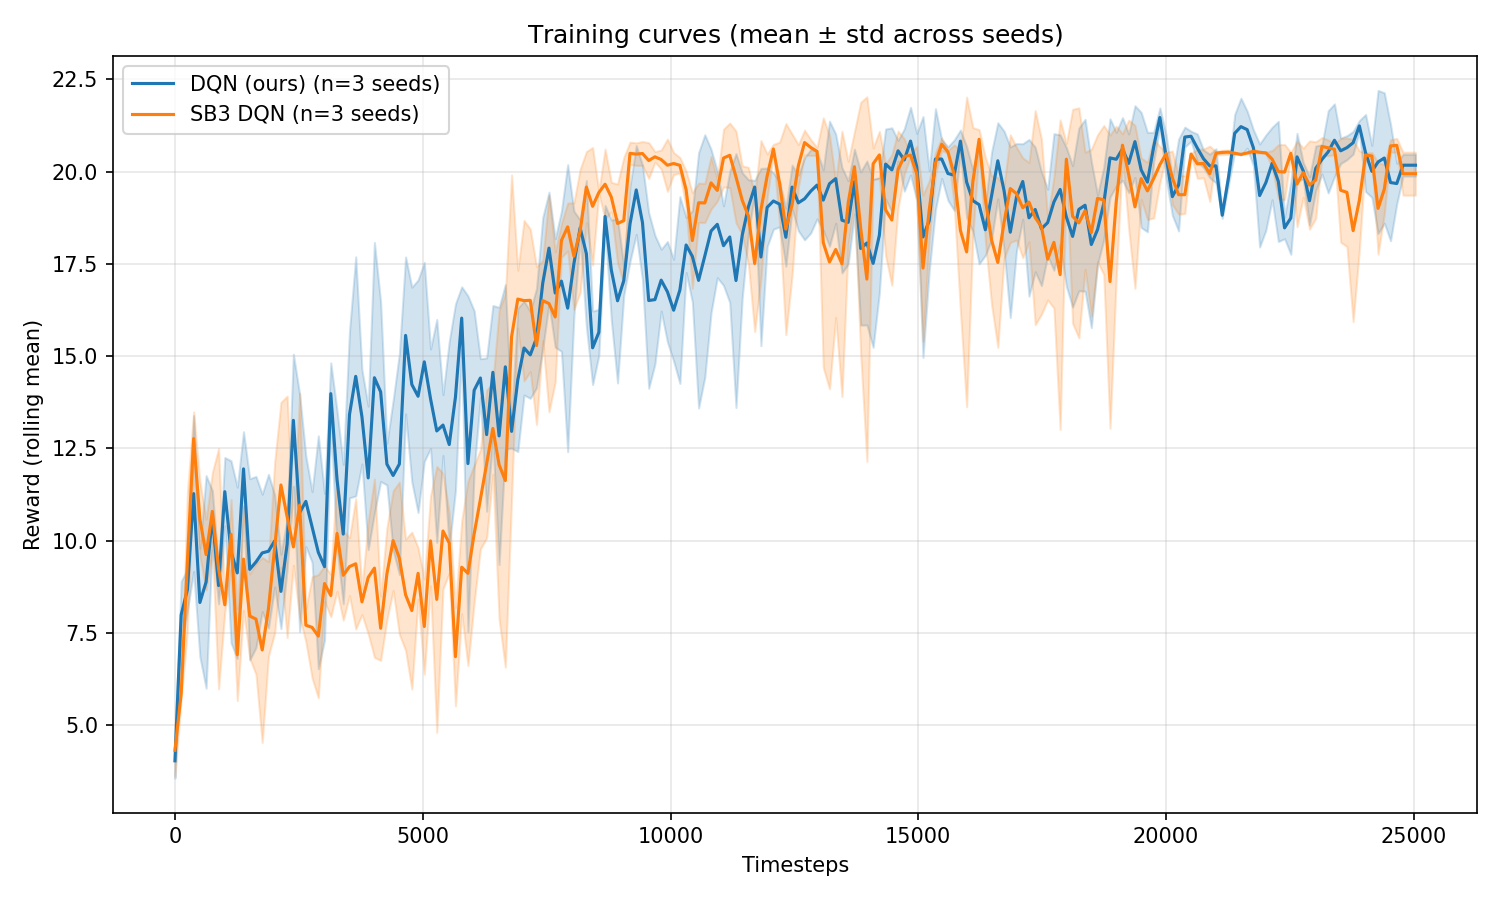
\includegraphics[width=0.85\textwidth]{../results_v3/figures/training_curves.png}

    \vspace{0.2cm}
    {\small Moyenne $\pm$ \'ecart-type sur 3 seeds (architectures identiques 256-256). Lissage par moyenne glissante (fen\^etre 10).}

    \vspace{0.2cm}
    \begin{itemize}
        \item Notre DQN converge vite ($\sim$5k timesteps) mais reste bruit\'e (crashes).
        \item SB3 d\'emarre plus lentement mais converge vers une politique \textbf{tr\`es stable}.
    \end{itemize}
\end{frame}

% ============================================================
% 9. EVALUATION QUANTITATIVE
% ============================================================
\begin{frame}{\'Evaluation quantitative (50 runs $\times$ 3 seeds)}
    \begin{table}
        \centering
        \begin{tabular}{lcccc}
            \toprule
            \textbf{Agent} & \textbf{Seed} & \textbf{Reward moy.} & \textbf{Std} & \textbf{Crashes} \\
            \midrule
            DQN (custom) & 52 & 19.81 & 4.52 & 9/50 (18\%) \\
            DQN (custom) & 53 & 18.99 & 5.51 & 12/50 (24\%) \\
            DQN (custom) & 54 & 20.76 & 3.44 & 8/50 (16\%) \\
            \textbf{DQN (custom)} & \textbf{total} & \textbf{19.85} & \textbf{4.63} & \textbf{29/150 (19\%)} \\
            \midrule
            SB3 DQN & 52 & 20.45 & 0.00 & 0/50 (0\%) \\
            SB3 DQN & 53 & 20.55 & 0.05 & 0/50 (0\%) \\
            SB3 DQN & 54 & 20.45 & 0.00 & 0/50 (0\%) \\
            \textbf{SB3 DQN} & \textbf{total} & \textbf{20.48} & \textbf{0.05} & \textbf{0/150 (0\%)} \\
            \bottomrule
        \end{tabular}
    \end{table}

    \vspace{0.2cm}
    SB3 : reward l\'eg\`erement sup\'erieure (+3\%), variance quasi-nulle, et \textbf{0 crash} vs 19\% pour notre DQN.
\end{frame}

% ============================================================
% 10. ANALYSE DES ECHECS
% ============================================================
\begin{frame}{Analyse des modes d'\'echec}
    \begin{columns}
        \begin{column}{0.5\textwidth}
            \textbf{Notre DQN (19\% de crashes)}

            \vspace{0.2cm}
            Deux patterns identifi\'es :
            \begin{itemize}
                \item \textbf{Crash pr\'ecoce} (steps 4--8) : changement de voie dans une voie occup\'ee juste apr\`es le reset. Reward tr\`es faible ($\sim$2--6).
                \item \textbf{Crash tardif} (steps 19--30) : collision en fin d'\'episode dans du trafic dense. Reward proche du max ($\sim$20).
            \end{itemize}
        \end{column}
        \begin{column}{0.5\textwidth}
            \textbf{SB3 DQN (0\% de crashes)}

            \vspace{0.2cm}
            Politique ultra-conservative :
            \begin{itemize}
                \item Reward quasi-constante ($\sim$20.45)
                \item Z\'ero crash sur 150 \'episodes
                \item Probablement : vitesse constante, pas de changement de voie
                \item S\^ur mais ne maximise pas la reward (pics \`a 24+ pour notre DQN)
            \end{itemize}
        \end{column}
    \end{columns}

    \vspace{0.3cm}
    \begin{block}{Compromis s\'ecurit\'e vs performance}
        SB3 privil\'egie la s\'ecurit\'e (0 crash) au d\'etriment du reward maximal. Notre DQN tente des man\oe uvres risqu\'ees qui parfois \'echouent mais atteignent des rewards plus \'elev\'ees.
    \end{block}
\end{frame}

% ============================================================
% 11. CHOIX DE DESIGN
% ============================================================
\begin{frame}{Choix de design}
    \begin{itemize}
        \item \textbf{Timesteps comme unit\'e commune :} permet une comparaison directe DQN vs SB3 sur le m\^eme axe. L'ancienne version utilisait des \'episodes (DQN) vs timesteps (SB3) $\Rightarrow$ incomparable.

        \vspace{0.2cm}
        \item \textbf{$\gamma = 0.99$ :} horizon lointain n\'ecessaire pour anticiper le trafic. Un $\gamma$ plus faible rendrait l'agent trop myope (ne planifie pas les d\'epassements).

        \vspace{0.2cm}
        \item \textbf{MLP 256-256 identique :} m\^eme architecture pour les deux agents. La v2 utilisait le \texttt{MlpPolicy} par d\'efaut (64-64) pour SB3 $\Rightarrow$ comparaison biais\'ee. La v3 corrige ce probl\`eme.

        \vspace{0.2cm}
        \item \textbf{Sauvegarde incr\'ementale (CSV) :} r\'esultats enregistr\'es apr\`es chaque seed. A sauv\'e nos donn\'ees quand le premier job cluster a \'et\'e tu\'e par SLURM.
    \end{itemize}
\end{frame}

% ============================================================
\section{Extension et Conclusion}
% ============================================================

% ============================================================
% 12. EXTENSION
% ============================================================
\begin{frame}{Extension : \textit{\`A compl\'eter}}
    \textbf{Direction envisag\'ee :} \textit{[Ex: Double-DQN / Prioritized Experience Replay / Safety-RL]}

    \vspace{0.3cm}
    \textbf{Hypoth\`ese :}
    \begin{itemize}
        \item \textit{[Ex: Double-DQN r\'eduit la surestimation des Q-values $\Rightarrow$ politique plus stable]}
    \end{itemize}

    \vspace{0.3cm}
    \textbf{Protocole exp\'erimental :}
    \begin{itemize}
        \item \textit{[Comparaison / ablation / variation contr\^ol\'ee]}
    \end{itemize}

    \vspace{0.3cm}
    \textbf{R\'esultats :}
    \begin{itemize}
        \item \textit{[\`A compl\'eter]}
    \end{itemize}
\end{frame}

% ============================================================
% 13. CONCLUSION
% ============================================================
\begin{frame}{Conclusion}
    \textbf{R\'esultats principaux :}
    \begin{itemize}
        \item Avec des architectures identiques (256-256), \textbf{SB3 surpasse notre DQN} : reward 20.48 vs 19.85, 0\% vs 19\% de crashes.
        \item SB3 apprend une politique conservatrice tr\`es stable. Notre DQN est plus agressif (pics \`a 24+) mais moins fiable.
    \end{itemize}

    \vspace{0.3cm}
    \textbf{Le\c{c}ons apprises :}
    \begin{itemize}
        \item L'importance d'une comparaison \'equitable : m\^eme architecture, m\^emes timesteps, m\^emes seeds. La v2 (architectures diff\'erentes) donnait des conclusions \textbf{oppos\'ees}.
        \item La robustesse de l'infrastructure (sauvegardes incr\'ementales, gestion du cluster).
        \item Les bugs silencieux (Monitor wrapper, observation space) peuvent invalider des r\'esultats sans signal d'erreur.
    \end{itemize}

    \vspace{0.3cm}
    \textbf{Perspectives :}
    \begin{itemize}
        \item Extension (Double-DQN, PER, Safety-RL)
        \item R\'eduire le taux de crash de notre DQN (reward shaping, exploration)
        \item G\'en\'eralisation \`a d'autres environnements (intersection, rond-point)
    \end{itemize}
\end{frame}

\end{document}
